\documentclass[11pt, a4paper, oneside]{book}

% Um sprache umzustellen
% \usepackage[ngerman]{babel}
\usepackage[english]{babel}

% Restliche Settings einfügen
\usepackage{Setup/settings}

% Einstellungen für Metainformation in PDF-Datei
\hypersetup{pdftitle={ESC241 Pion and Muon lifetime},
            pdfauthor={Till Böhringer, Lucien Käser, Marc Urech, Richard Salnikov}}

% Was im Footer stehen soll, ifoot -> links, cfoot -> mitte
\ifoot{Pion and muon lifetimes}
\cfoot{ESC241}

% Allgemeine weite um alle Figures darauf zu beziehen
\newcommand\Plotwidth{0.8}
\newcommand\Bilderwidth{0.8}

% Setup wie siunix zahlen schreibt
\sisetup{group-separator = {'}, group-digits = integer}

% some stuff to make writing this report easiert
\newcommand{\electron}{$e^{-}$}
\newcommand{\pion}{$\pi^{-}$}
\newcommand{\muon}{$\mu^{-}$}

\lstset{language=python,
       basicstyle=\footnotesize\ttfamily,
  }

\begin{document}

% Bitte Titlepage noch bearbeiten falls nötig
\newgeometry{bottom=1cm, top=4cm} % die Abstände von oben und unten korrigieren
\begin{titlepage}
    \setlength{\headheight}{0cm}
	%\centering
	\includegraphics[width=0.45\textwidth]{\thelogofilename}\par\vspace{1cm}
    % \includesvg[width=0.45\textwidth]{\thelogofilename}\par\vspace{1cm}
	
	\centering
	
	{\bfseries\LARGE University of Zurich\par}
	\vspace{0.7cm}
	
	{\Huge\bfseries Pion and muon lifetimes\par}
	\vspace{0.7cm}

	{\LARGE Data analysis 2025 \par Group project IV \par }
	\vfill

    {\large Authors:\par\vspace{0.2cm}}
	{\Large\itshape Till Böhringer\\ \href{mailto:tillnils.boehringer@uzh.ch}{tillnils.boehringer@uzh.ch} \par
	\Large\itshape Lucien Käser\\ \href{mailto:luciendarian.kaeser@uzh.ch}{luciendarian.kaeser@uzh.ch} \par
	\Large\itshape Marc Urech\\ \href{mailto:marcandre.urech@uzh.ch}{marcandre.urech@uzh.ch} \par
	\Large\itshape Richard Salnikov\\ \href{mailto:richardivan.salnikov@uzh.ch}{richardivan.salnikov@uzh.ch} \par}
	\vfill

	
	{\large Lecturer:\par\vspace{0.2cm}}
	{\Large Patrick Owen}
	\vfill
	\vfill

% Bottom of the page
	{\large \today\par}
\end{titlepage}
\restoregeometry % das das restliche Dokument wieder die normale Geometrie hat
\frontmatter

\tableofcontents
\mainmatter

\chapter{Abstract}
% Short summary: goal, method, main results, ... 

\chapter{Introduction}
% what we want to do
In this project, a simplified simulation of an experiment for measuring the lifetimes of charges pions (\pion) and muons (\muon) will be performed.

% problem description
\section{Motivation}
Negatively charged pions (\pion) are composite particles, that consist of a down quark and an up antiquark. They are unstable and decay predominantly to a muon (\muon) and a muon-antineutrino ($\bar{v_{\mu}}$). The muon, a heavier partner of the electron, is also unstable and decays into an electron (\electron), a muon-neutrino ($v_{\mu}$) and an electron antineutrino ($\bar{v_{e}}$). Neglecting any experimental effects, the time distribution of the \electron produced in the decay chain is given by

\begin{equation}
    N(t) = \frac{N_0}{\tau_{\mu} - \tau_{\pi}}  \left[ \exp{-\frac{t}{\tau_{\mu}}} - \exp{-\frac{t}{\tau_{\pi}}} \right]
    \label{eq:decay_chain_equation}
\end{equation}

Where $\tau_{\mu}$ and $\tau_{\pi}$ are the mean lifetimes of the \muon and \pion respectively. A measurement of this time distribution allows extracting times for $\tau_{\mu}$ and $\tau_{\pi}$.

\section{Setup}

The basic elements of the corresponding real experiment are shown in Figure \ref{fig:experimental_setup} negatively charged pion (\pion) is stopped in the third scintillator. The emitted electron (\electron) is then detected in the fifth scintillator. The time difference between the moment the \pion is stopped in the third scintillator and the \electron is detected in the fifth scintillator is recorded. A spectrum of time differences for many such events will allow for an estimation of the half life times of the \pion ($\tau_{\pi}$) and the \muon ($\tau_{\mu}$).

\begin{figure}[h]
\begin{center}
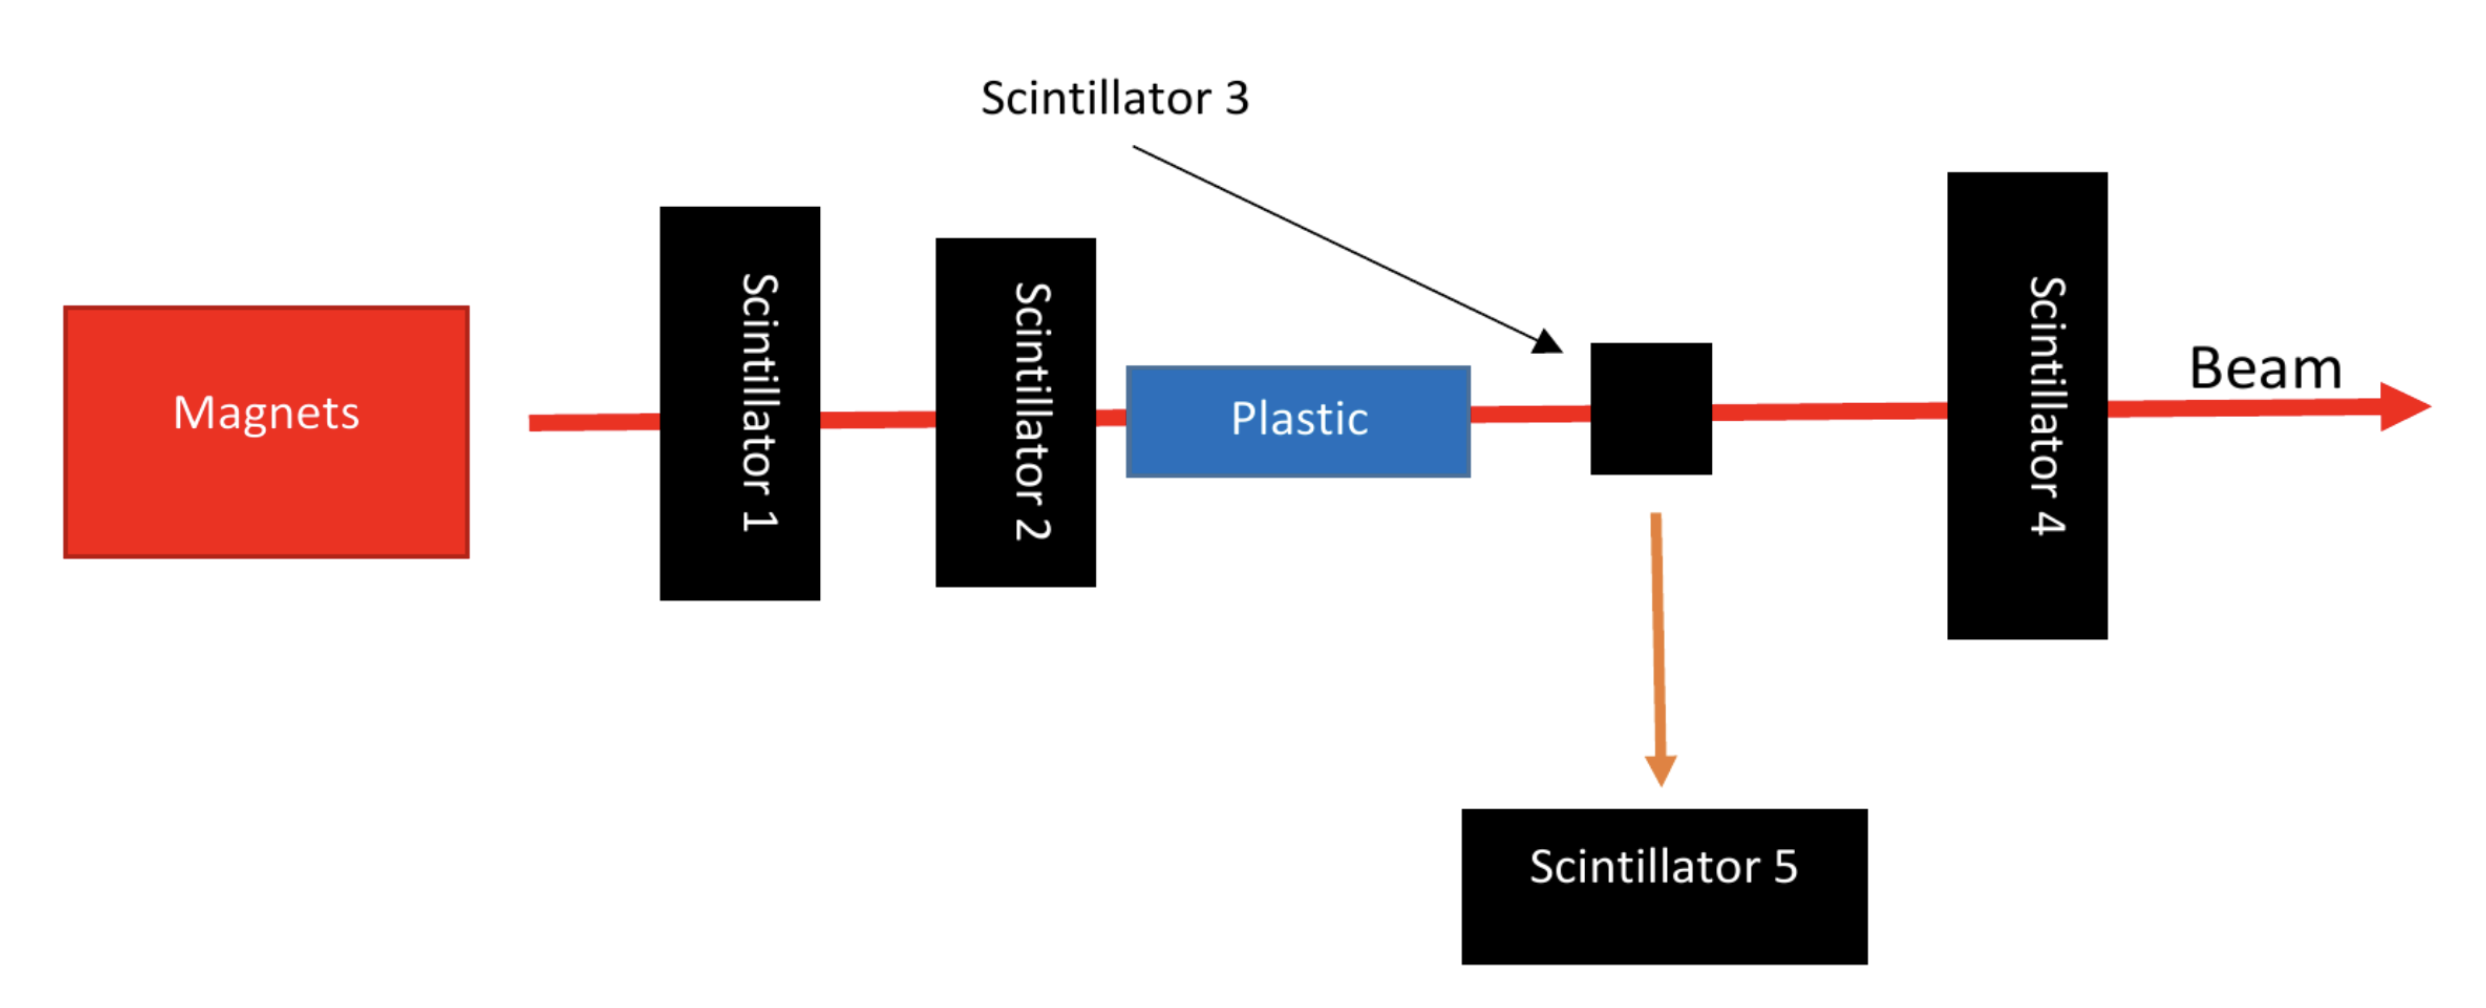
\includegraphics[width=0.7\textwidth]{images/experimental_setup.png}
\end{center}
\caption{Simplified sketch of the setup of the experiment (from the project documentation). A beam containing \pion passes through scintillators 1 and 2 and a piece of plastic to slow them down, such that they stop in scintillator 3. Scintillator 4 is a counter to reject events in which the beam particle was not stopped in scintillator 3. Electron \electron created in the decay chain are detected in scintillator 5. The signal from scintillator 3 starts a clock, the signal from scintillator 5 stops it.}
\label{fig:experimental_setup}
\end{figure}

\section{Validation of the simulation using the pull}
\begin{equation}
    \si{pull} = \frac{\bar{\tau} - \tau}{\sigma_{\bar{\tau}}}
    \label{eq:pull}
\end{equation}
The pull allows for a check of the estimated values. The pull of many simulations should follow a gaussian distribution with a mean of 0 as well as a standard deviation of 1. A deviation from these values can be an indication for the following problems:

Deviations in the mean value from 0, indicate a bias in the estimation of the lifetimes. Whereas a standard deviation larger or smaller than 1 indicate an under- / overestimation of the uncertainties. 

\section{Computational implementation}
In this project, a simplified version of the experiment is simulated. At first, \num{10000} decay time measurements are simulated using the known values of the lifetimes of the \pion and \muon. This corresponds to the time difference between the moment the \pion is stopped in scintillator 3 and the \electron is detected in scintillator 5. Working with these simulated decay times, the goal is to extract the lifetimes of the \pion and \muon.

For the implementation python 3.10.11 is used, with the following packages:
\begin{itemize}
    \item numpy 2.0.0
    \item matplotlib 3.9.2
    \item scipy 1.14.1
    \item pandas 2.2.3
\end{itemize}
All used packages are freely available under an open-source license. 
The full implementation of the simulation as well as this documentation is available on \cite{GitHub}.

% goal of the simulation
% short theoretical background

\FloatBarrier
\chapter{Methods}

In this chapter we go over the simulations we have done, at first a simple simulation and second a more realistic example.
In this chapter, the two performed simulations are described. The first simulation is a simpler version of the second one. Latter of which is a bit more realistic, as it includes the finite time resolution of the apparatus. 

\section{Simple simulation}
The goal of the first simulation is to simulate the decay of \pion and \muon without taking the finite time resolution of the apparatus into account. The simulation for this will take the following steps:
\begin{itemize}
    \item Generated \num{10000} decay times according to the equation \ref{eq:decay_chain_equation} using the knows values of the lifetimes of the \pion and \muon.
    \item Perform a binned maximum likelihood fit to the histogram to extract the estimates for the lifetimes of the \pion and \muon, as well as the uncertainties.
    \item Repeat the simulation \num{100} times to get a distribution of the estimates, to calculate the standard deviation.
    \item Validation of the estimates using the pull, as defined in equation \ref{eq:pull}.
\end{itemize}
% d\tau_{\pi}ription of the simulation model
% assumptions made
% algorithms or numerical methods used
% software / tools used

\section{Implementation of the simple simulation}

\subsection{Simulation of the decay times}
For the simple simulation, equation \ref{eq:decay_chain_equation} is used to generate \num{10000} decay times using the known values of the lifetimes of the \pion and \muon. These values are given by:

\pion Mean lifetime: \qty{2.6033(0.0005)e-8}{\s} \\
\muon Mean lifetime: \qty{2.1969811(0.0000022)e-6}{\s} \\
reference: \cite{ParticleDataGroup:2024cfk}

%TODO: add a plot of the distribution without anything in it

The decay times are generated using the accept-reject method. For this, a random point on the domain of the distribution is generated (t, y). If the generated point is below the distribution, it is accepted, if not, it is rejected. This is done until the target number of points is reached. 
The decay time $t$ is generated using a uniform distribution between 0 and \qty{1}{\s}. The count $y$ is also drawn from a uniform distribution between \qty{0} and the maximum value of the target distribution $max(N(t))$

The random points generated are shown in figure \ref{fig:histogram}. The overlaid distribution is given by equation \ref{eq:decay_chain_equation} using the know values.


\begin{figure}[H]
    \centering
    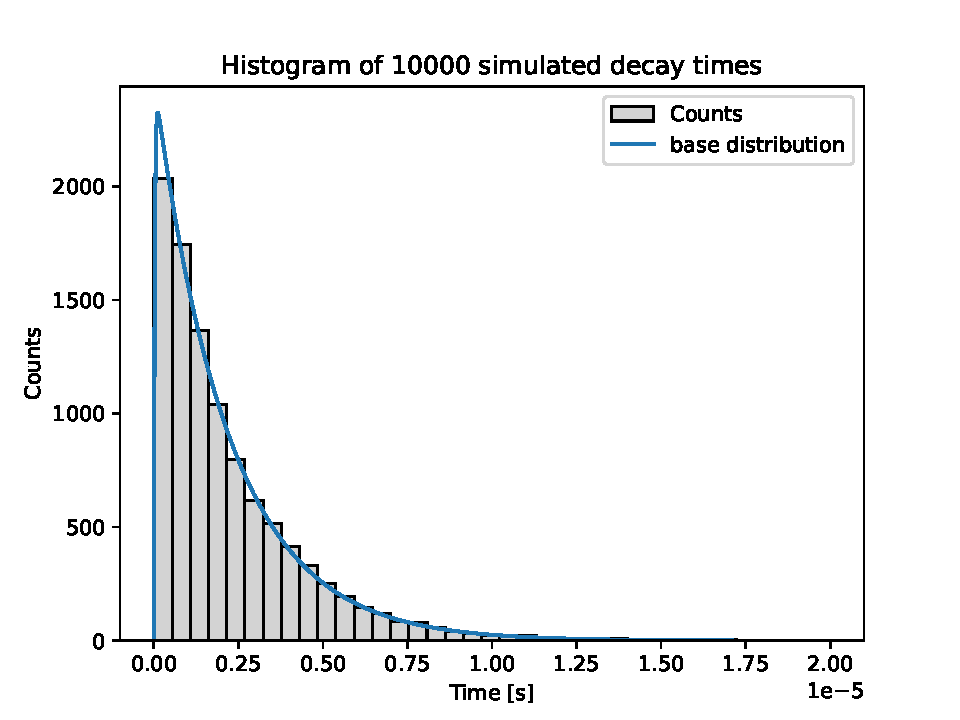
\includegraphics[width=\Plotwidth\textwidth]{images/simulated_decay_histogram.pdf}
    \caption{The histogram generated using accept-reject method.}
    \label{fig:histogram}
\end{figure}

\subsection{Estimation of the lifetimes}
Next a binned-maximum-likelihood was performed on the histogram. For this the likelihood was calculated ans minimized using the combination of scipy's minimization function as well as a custim markov-chain-monte-carlo minimizer. Although this method worked, it presented with multiple problems: The entire estimation process took a long time, as the mcmc-method required to run for some \num{10000} iterations to get a good estimate. Furthermore it presented with a bias on the lifetime of the \pion, as can be seen in figure \ref{fig:pull_likelihood_method}. 

\begin{figure}[H]
    \centering
    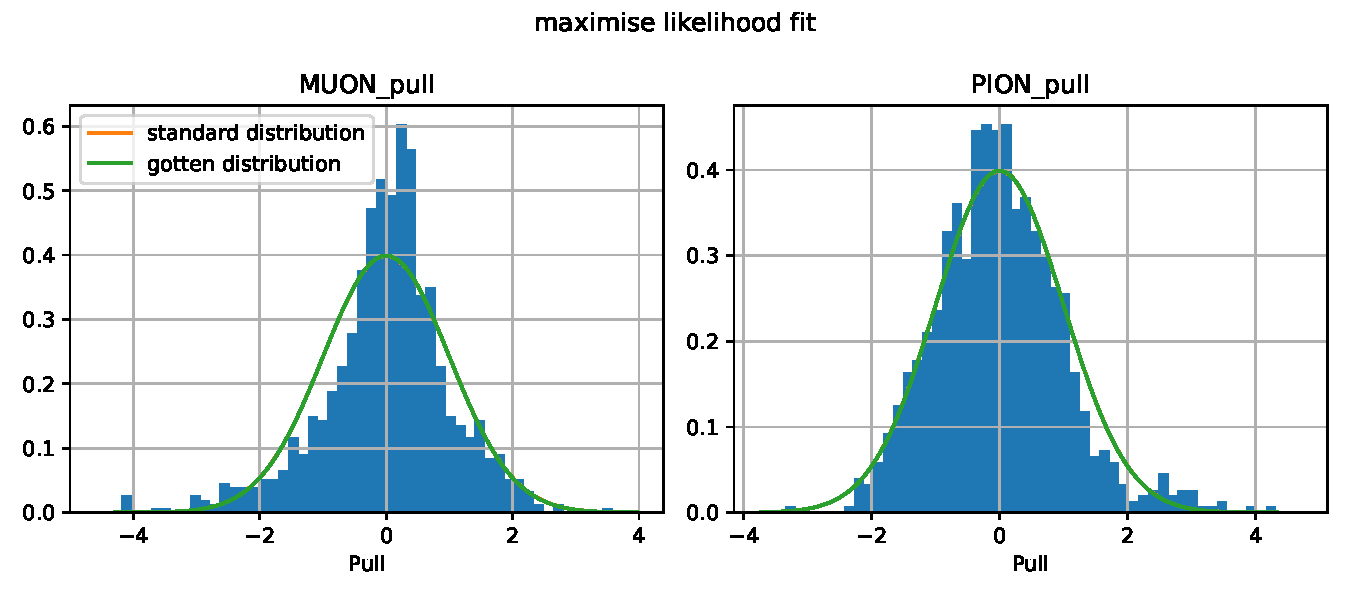
\includegraphics[width=\Plotwidth\textwidth]{images/estimators_pull_likelihood.pdf}
    \caption{The pull of the estimated lifetimes using the binned maximum likelihood method.}
    \label{fig:pull_likelihood_method}
\end{figure}

To improve the estimation, the least squared method was also considered. Using the same formula and data, it returned better estimations, as can be seen in figure \ref{fig:comparison_estimators}. The least squares method was implemented using the \lstinline|curve_fit| function from the scipy package and was also done on the bins. 


%Next we fitted back on the generated histogram the distribution, getting values for the lifetimes and corresponding uncertainties. The fitting was supposed to be done via a maximum likelihood fit, but as can be seen in figure \ref{fig:comparison_estimators}, the least squares method gives better results than the maximum likelihood fit. In figure \ref{fig:comparison_estimators} the maximum likelihood fit is implemented with the SciPy \lstinline|minimize| function, the least squares fit is done with the SciPy \lstinline|curve_fit| function and the full is a stack of fitters from \lstinline|dual_annealing| over a local \lstinline|minimize| to a custom markov-chain minimizer.

\begin{figure}[H]
    \centering
    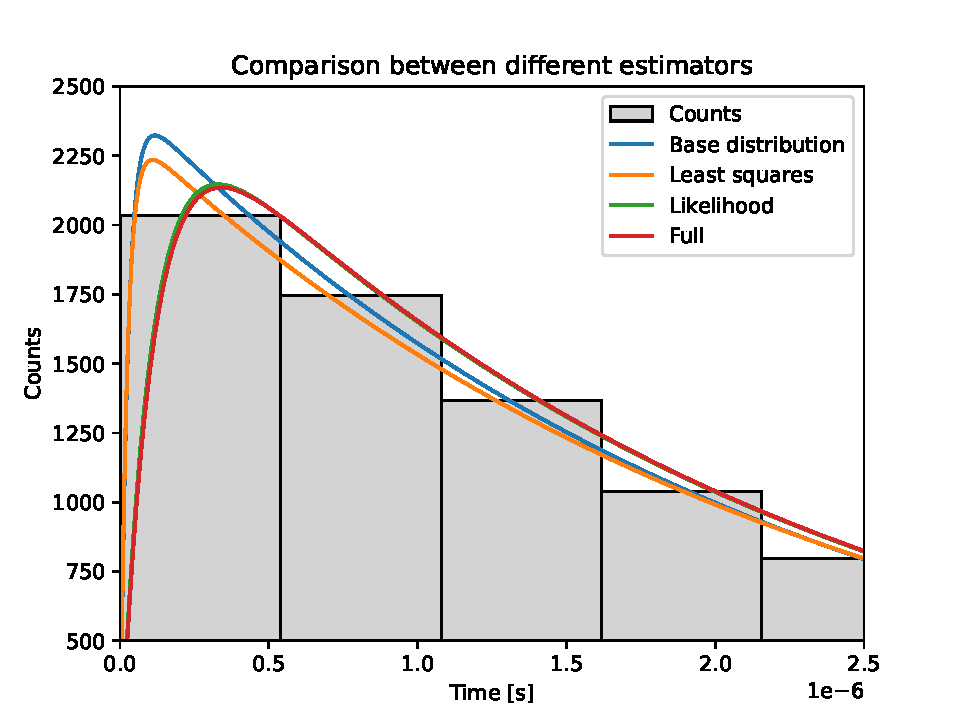
\includegraphics[width=\Plotwidth\textwidth]{images/comparison_estimators.pdf}
    \caption{Comparison between different estimators and the base distribution, overlaid on the histogram.}
    \label{fig:comparison_estimators}
\end{figure}

As the least squared method returns better estimations for the lifetimes, it will also be used for the second simulation as an extention to the binned maximum likelihood method.

As can be seen in figure \ref{fig:comparison_estimators} the best representation to the base distribution gives the least squares fit, which we will use for the further exercises.

\subsection{Uncertainties of the estimators}
For the estimation of the uncertainties, two different methods were used. 
\begin{itemize}
    \item For the method using the binned maximum likelihood, the uncertainties were calculated by finding the points, where the likelihood is \qty{0.5} away from the minimum. This is done by using the minimal value of the likelihood and subtracting \qty{0.5} from it. Then the roots of the likelihood function were calculated using newton-raphons method. 
    \item For the least squared method, the uncertainties were calculated using the covariance matrix, which is returned as part of the \lstinline{minimization_results} object. The uncertainties are given by the root of half of the diagonal elements of the covariance matrix.
\end{itemize}


\chapter{Results}
% present key results (plots, tables, values)
% explain findings objectively, without interpretation

\chapter{Discussion}
% interpretation of the results
% compare with theory or expectations
% sources of error, limitations by the simulation

% \clearpage
% \phantomsection
% \addtocounter{chapter}{1}
% \addcontentsline{toc}{chapter}{\protect\numberline{\thechapter}{\listtablename}}
% \listoftables

% \clearpage
% \phantomsection
% \addtocounter{chapter}{1}
% \addcontentsline{toc}{chapter}{\protect\numberline{\thechapter}{\listfigurename}}
% \listoffigures

% \printbibliography[heading=bibintoc, title={Quellenverzeichnis}]
% \printbibliography[heading=bibintoc]
\IfLanguageName{ngerman}{\printbibliography[heading=bibintoc, title={Quellenverzeichnis}]}{\printbibliography[heading=bibintoc]}

\listoftables

\listoffigures

% \addtocontents{toc}{\protect\newpage}

\end{document}